\documentclass[12pt,a4paper]{article}

\usepackage[T1]{fontenc}
\usepackage[utf8]{inputenc} % Use UTF-8 encoding for input
\usepackage[french]{babel}

\usepackage{lmodern}	
\usepackage{amsmath}
\usepackage{amsfonts}
\usepackage{amssymb}
\usepackage{graphicx}
\usepackage{xcolor}
\usepackage{mathtools}
\usepackage{fancyhdr}
\usepackage{enumitem}
\usepackage{tcolorbox}
\usepackage{colortbl}
\usepackage{multirow}
\usepackage{stmaryrd}
\usepackage{dsfont}
\usepackage{tikz}
\usepackage{hyperref}
\usepackage[upgreek]{txgreeks}
\usepackage{algpseudocode}
\usepackage{algorithm}
\usepackage[text={15cm,24.5cm},centering]{geometry}


% Définir le texte affiché en fin de page
\pagestyle{fancy}
\fancyhf{}  % Clear the default headers and footers
\rfoot{\hrule
    \vspace{0.3cm}
    \noindent\textsf{Résolution de systèmes linéaires issus d'EDP}
    \hfill \thepage
}
\renewcommand{\headrulewidth}{0pt}

\title{\vspace{4cm}
        Rapport \\
        \vspace{1cm} \textbf{TP1 : Méthodes GMRES et FOM} \\ 
        \vspace{4cm} 
}

\author{\textit{Réalisé par} \vspace{0.5cm}\\
         \textbf{Mathilde Ferreira} \\
        \textbf{Félix Foucher de Brandois}
}
        
\date{\vfill
        \textit{ENSEEIHT} - 
        \textit{Formation ModIA, 5$^{e}$ année}
        \hfill
        \textit{2024-2025} \\
        \vspace{1cm}
}


\begin{document}

\begin{figure}[t]
    \centering
    
\includegraphics[width=7cm]{src/inp_n7.png}
    \hfill
    
\includegraphics[width=5.5cm]{src/insa_toulouse.png}
\end{figure}


\maketitle
\thispagestyle{empty}

\newpage


\section{Introduction}
\noindent On cherche à résoudre le système linéaire : $Ax = b$ \\
avec $A \in \mathbb{R}^{n \times n}$ une matrice creuse, symétrique définie positive, $b \in \mathbb{R}^{n}$ et $x \in \mathbb{R}^{n}$. \\

Pour cela on considère les méthodes itératives GMRES et FOM et on s’intéressera aux historiques de convergence de ces méthodes en termes de norme relative du résidu, définie par :
$$
\eta_b^N(x_m) = \frac{\|b - Ax_m\|}{\|b\|}.
$$

où $x_m$ représente la solution approchée à l'itération $m$.
Les itérations sont arrêtées lorsque cette norme relative du résidu atteint un seuil $\epsilon$ prédéfini ou lorsqu'un nombre maximum d'itérations est atteint. \\

Dans ce rapport, nous présentons les résultats obtenus, notamment le nombre d'itérations nécessaires pour atteindre la convergence et la précision obtenue pour chaque méthode.
Nous illustrons également l'évolution de la norme du résidu au fil des itérations et comparons ces résultats avec ceux obtenus par la fonction \texttt{gmres} de MATLAB.
On s'intéresse également à l'impact de la tolérance $\epsilon$ sur la convergence des méthodes GMRES et FOM.


\section{Algorithme GMRES}

Nous avons adapté l'algorithme GMRES (Generalized Minimal Residual) pour qu'il s'arrête lorsque l’itéré courant vérifie le critère de convergence (erreur inverse relative inférieure à une certaine tolérance) ou lorsque le nombre d’itérations est supérieur au nombre d’itérations maximum accepté.

\begin{algorithm}
    \caption{GMRES - Modified Gram-Schmidt (MGS) variant}
    \begin{algorithmic}[1] % [1] pour la numérotation des lignes
        \State Set the initial guess $x_0$
        \State Compute $r_0 = b - Ax_0$, $\beta = \|r_0\|$
        \State Set $v_1 = r_0 / \beta$
        \State Compute relative residual: $\text{relres} = \beta / \|b\|$
        \State Initialize iteration counter: $j = 1$
        \While{$\text{relres} > \text{tol}$ \textbf{and} $j \leq \text{maxit}$}
            \State Compute $w_j = Av_j$
            \For{$i = 1$ \texttt{to} $j$}
            \State $h_{i,j} = v_i^T w_j$
            \State $w_j = w_j - h_{i,j} v_i$
            \EndFor
            \State Compute $h_{j+1,j} = \|w_j\|$
            \State Normalize: $v_{j+1} = w_j / h_{j+1,j}$
            \State Compute QR decomposition: $Q, R = \text{qr}(\bar{H})$
            \State Compute $g = Q^T \beta e_1$
            \State Solve the least-squares problem: $y = \arg \min \|g - Ry\|$
            \State Compute residual estimate: $r_j = |g_{j+1}|$
        \EndWhile
        \State Compute solution: $x_m = x_0 + V_m y_m$
    \end{algorithmic}
\end{algorithm}

Pour éviter de calculer le résidu à chaque itération, nous faisons l'estimation de la norme du résidu en utilisant la relation suivante :
$$
r_j = |g_{j+1}|
$$
où $g_{m+1}$ est le dernier élément de $g$ après la résolution du problème de moindres carrés.


\section{Algorithme FOM}

Nous avons également implémenté l'algorithme FOM (Full Orthogonalization Method) en remplaçant le calcul du résidu par l'estimation de la norme du résidu :
$$
r_j = h_{j+1,j} |e_j^T y_j|
$$

\begin{algorithm}
    \caption{FOM - Full Orthogonalization Method}
    \begin{algorithmic}[1] % [1] pour la numérotation des lignes
        \State Set the initial guess $x_0$
        \State Compute $r_0 = b - A x_0$, $\beta = \|r_0\|$
        \State Set $v_1 = r_0 / \beta$
        \State Compute relative residual: $\text{relres} = \beta / \|b\|$
        \State Initialize iteration counter: $j = 1$
        \While{$\text{relres} > \text{tol}$ \textbf{and} $j \leq \text{maxit}$}
            \State Compute $w_j = A v_j$
            \For{$i = 1$ \textbf{to} $j$}
                \State $h_{i,j} = v_i^T w_j$
                \State $w_j = w_j - h_{i,j} v_i$
            \EndFor
            \State Compute $h_{j+1,j} = \|w_j\|$
            \State Normalize: $v_{j+1} = w_j / h_{j+1,j}$
            \State Compute $y_j = H^{-1} \beta e_1$
            \State Compute residual estimate: $r_m = h_{j+1,j} |e_j^T y_j|$
        \EndWhile
        \State Compute solution: $x_m = x_0 + V_m y_m$
    \end{algorithmic}
\end{algorithm}

\section{Résultats}

\begin{table}[H]
    \centering
    \begin{tabular}{|c|c|c|c|c|}
    \hline
    \rowcolor{gray!20} \textbf{Matrice} & \textbf{Taille de la matrice} & \textbf{Méthode} & \textbf{Nb itérations} & \textbf{Erreur relative} \\
    \hline
    \multirow{3}{*}{\texttt{mat1.mat}} & \multirow{3}{*}{573} & FOM & 174 & 1.99e-08 \\
    \cline{3-5}
     &  & GMRES & 172 & 4.90e-08 \\
    \cline{3-5}
     &  & GMRES matlab & 172 & 4.90e-08 \\
    \hline
    \multirow{3}{*}{\texttt{pde225\_5e-1.mat}} & \multirow{3}{*}{225} & FOM & 56 & 1.26e-07 \\
    \cline{3-5}
     &  & GMRES & 55 & 2.41e-07 \\
    \cline{3-5}
     &  & GMRES matlab & 55 & 2.41e-07 \\
    \hline
    \multirow{3}{*}{\texttt{hydcar20.mat}} & \multirow{3}{*}{99} & FOM & 99 & 2.33e-12 \\
    \cline{3-5}
     &  & GMRES & 99 & 2.69e-12 \\
    \cline{3-5}
     &  & GMRES matlab & 99 & 4.29e-12 \\
    \hline
    \end{tabular}
    \caption{Résultats pour $eps=10^{-6}$}
\end{table}

Les résultats obtenues avec GMRES sont très proche de sa version matlab ce qui suggère que notre implémentation est correcte. \\

Pour toutes les matrices, GMRES (et sa version Matlab) converge légérement plus rapidement que FOM en termes de nombre d'itérations, mais les erreurs relatives sont souvent légèrement plus grandes pour GMRES.
Cependant les erreurs relatives restent très faible ce qui indique une bonne convergence des méthodes.

Les performances des méthodes dépendent des caractéristiques de la matrice. \\
Pour des matrices plus petites comme \texttt{hydcar20.mat}, les erreurs sont extrêmement faibles, tandis que pour des matrices plus grandes comme \texttt{mat1.mat}, elles sont plus élevées. \\
Dans le cas de \texttt{hydcar20.mat}, le nombre d'itération est égale au la taille de la matrice, ainsi la convergence a été atteinte au maximum d'itérations. \\

La figure \ref{fig:residu} illustre l'évolution de la norme du résidu en fonction des itérations pour les trois matrices considérées : \texttt{mat1.mat}, \texttt{pde225\_5e-1.mat} et \texttt{hydcar20.mat}.

\begin{figure}[H]
    \centering
    \begin{minipage}{0.45\textwidth}
        \centering
        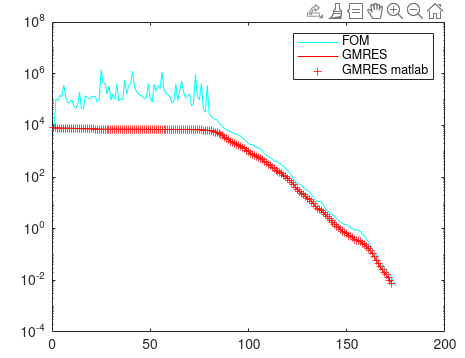
\includegraphics[width=\textwidth]{src/mat1.png}
        \caption{mat1}
    \end{minipage}
    \hfill
    \begin{minipage}{0.45\textwidth}
        \centering
        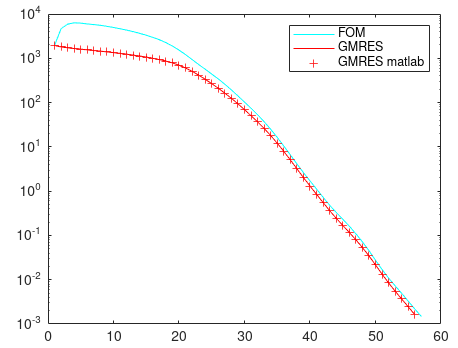
\includegraphics[width=\textwidth]{src/pde.png}
        \caption{pde225\_5e-1}
    \end{minipage}
    \hfill
    \begin{minipage}{0.45\textwidth}
        \centering
        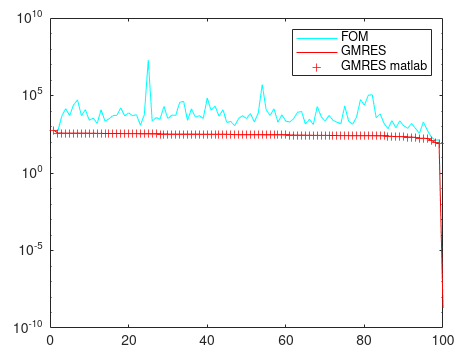
\includegraphics[width=\textwidth]{src/hyd.png}
        \caption{hydcar20}
    \end{minipage}
    \caption{Evolution du résidu en fonction des itérations}
    \label{fig:residu}
\end{figure}

On remarque que la courbe de GMRES s'aligne avec celle de GMRES de matlab.
On observe bien une convergence du résidu avec FOM et GMRES pour toutes les matrices.
La méthode FOM est parfois bruité dans ses premières itérations, elle semble plus sensible  aux propriétés des matrices que la méthode GMRES. \\


\noindent \textbf{Impact de la tolérance $\epsilon$ sur la convergence} \\
On a fait varier la tolérance afin de voir son impact sur la convergence des méthodes GMRES et FOM.

\begin{figure}[H]
    \centering
    \begin{minipage}{0.45\textwidth}
        \centering
        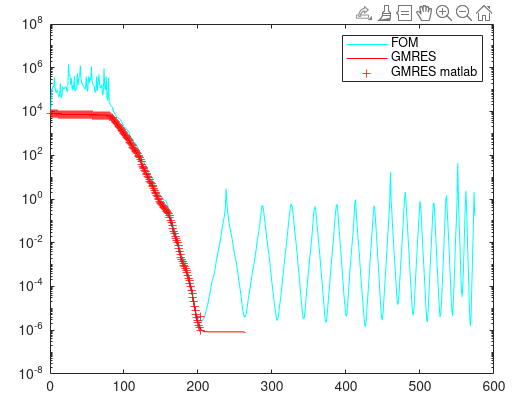
\includegraphics[width=\textwidth]{src/mat1_10.png}
        \caption{mat1 avec $eps=10^{-10}$}
    \end{minipage}
    \hfill
    \begin{minipage}{0.45\textwidth}
        \centering
        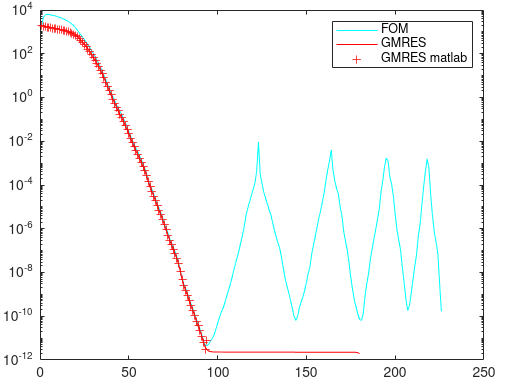
\includegraphics[width=\textwidth]{src/pde_15.png}
        \caption{pde225\_5e-1 avec $eps=10^{-15}$}
    \end{minipage}
    \hfill
    \begin{minipage}{0.45\textwidth}
        \centering
        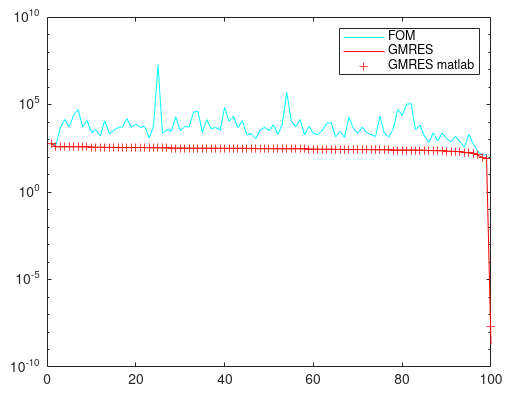
\includegraphics[width=\textwidth]{src/hyd_12.png}
        \caption{hydcar20 avec $eps=10^{-12}$}
    \end{minipage}
    \caption{Evolution du résidu en fonction des itérations}
    \label{fig:residu_eps}
\end{figure}

On observe que lorsque la tolérance est trop faible, les méthodes ne convergent pas. \\


\end{document}